\section{Altri Approcci}

\subsection{Modello ad Agente su Spazio Continuo}

L'approccio iniziale prevedeva la modellazione di una popolazione 
attraverso l'utilizzo di uno spazio di modello continuo. 
Gli agenti sarebbero stati rappresentati come individui reali, 
con un'effettiva presenza all'interno dello spazio. Questo spazio 
di modello continuo poteva essere visualizzato come una griglia di 
dimensioni $N \times M$ in cui gli agenti venivano posizionati in 
modo casuale e rappresentati come punti colorati.

\begin{minipage}{\linewidth}
    \centering
    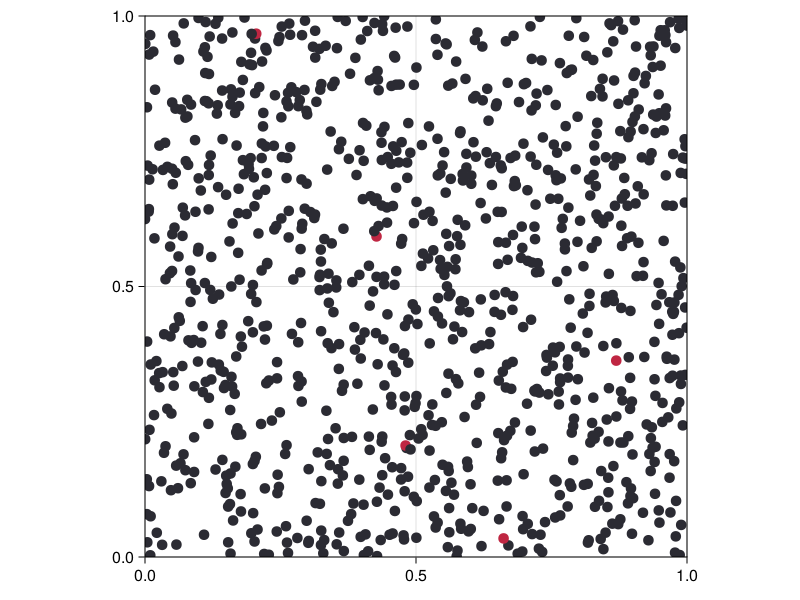
\includegraphics[width=\textwidth]{img/ball-covid.png}
    \captionof{figure}{Esempio del modello modellato su spazio continuo}
    \label{fig:ball_covid}
\end{minipage}

\begin{minipage}{\linewidth}
    \centering
    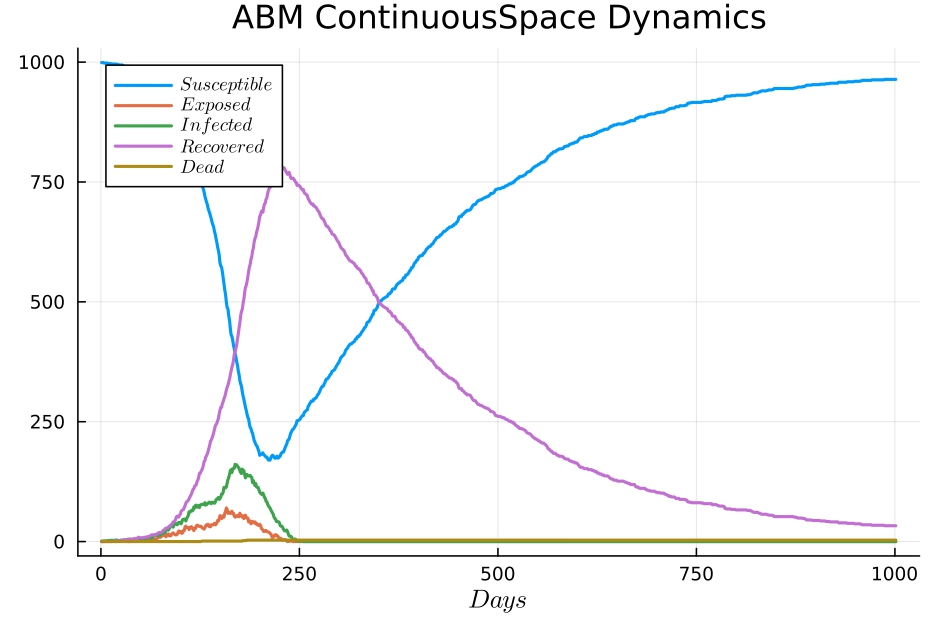
\includegraphics[width=\textwidth]{img/plot_abm_continuousspace.jpg}
    \captionof{figure}{Esempio del comportamento delle curve nel modello continuo}
    \label{fig:seir_curve_continuous}
\end{minipage}

Questo approccio prendeva spunto dalla fisica delle palline da 
biliardo per modellare le interazioni tra gli agenti all'interno 
dello spazio del modello. Ogni agente poteva casualmente infettare 
un vicino solo se interagivano, e questa interazione veniva modellata 
come un urto elastico tra corpi, anche se non rappresentava un vero 
simulatore di urti elastici, bensì ne prendeva spunto.

Tuttavia, questo approccio è risultato eccessivamente granulare e 
poco adatto agli obiettivi del progetto. Inoltre, richiedeva una 
quantità considerevole di risorse computazionali e tempo, il che 
ha portato alla sua sostituzione con un approccio più astratto e flessibile.
\newpage

\subsection{Modello ad Agente con Spazio a Grafo e Modellazione Singolo Agente}

Un secondo approccio è stato progettato per consentire un maggiore 
controllo sullo spazio di modello e la sua evoluzione locale, 
piuttosto che sugli agenti individuali. Tuttavia, questo approccio 
ha incontrato problemi significativi, tra cui tempi di esecuzione 
estremamente lunghi e un comportamento delle curve epidemiologiche 
completamente divergente rispetto al modello SEIR deterministico. 
Questo comportamento anomalo è stato osservato in presenza di variazioni 
nel parametro $R_0$, e la causa rimane sconosciuta.

\begin{minipage}{\linewidth}
    \centering
    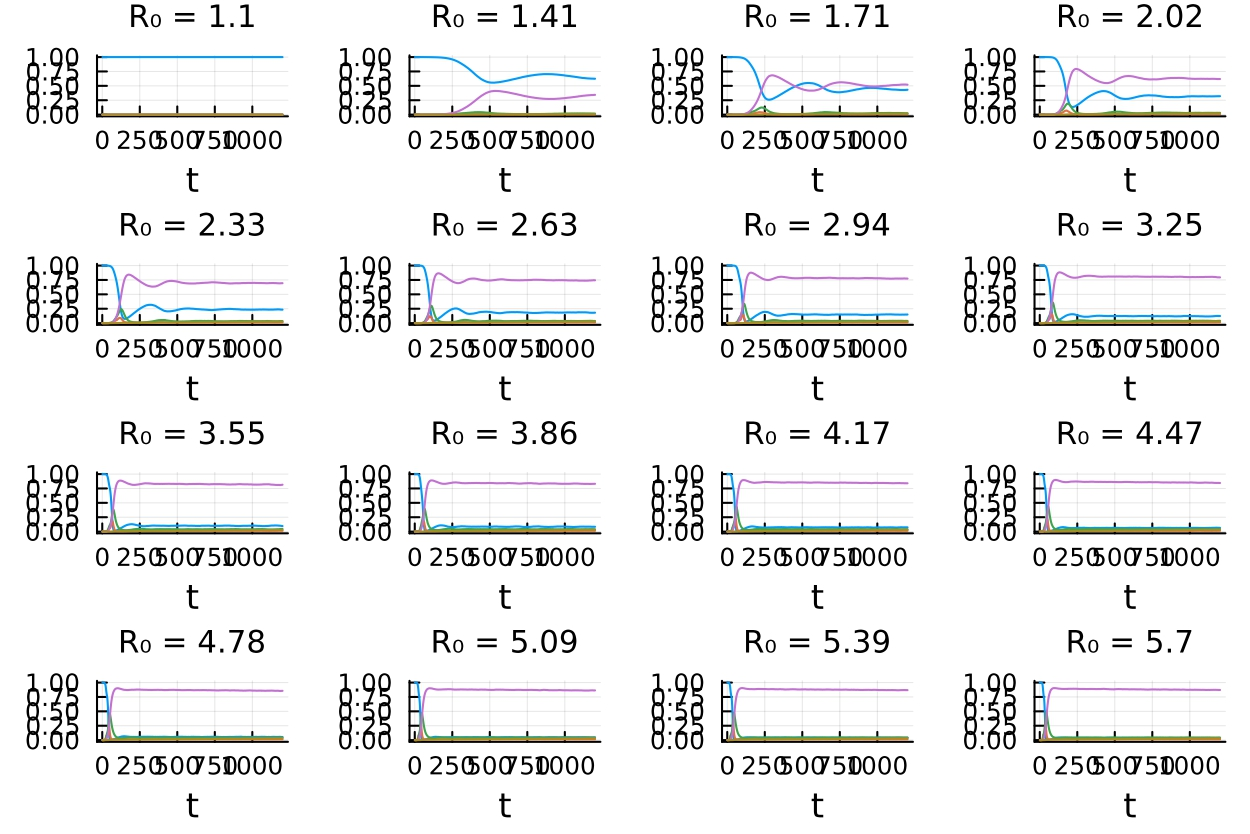
\includegraphics[width=\textwidth]{img/COMPARISON DIFFERENT R0 VALUE_2023-06-29.jpg}
    \captionof{figure}{Comportamento modello ABM su spazio a grafo al variare del parametro $R_0$}
    \label{fig:strange_behaviour_R0_abm}
\end{minipage}

\begin{minipage}{\linewidth}
    \centering
    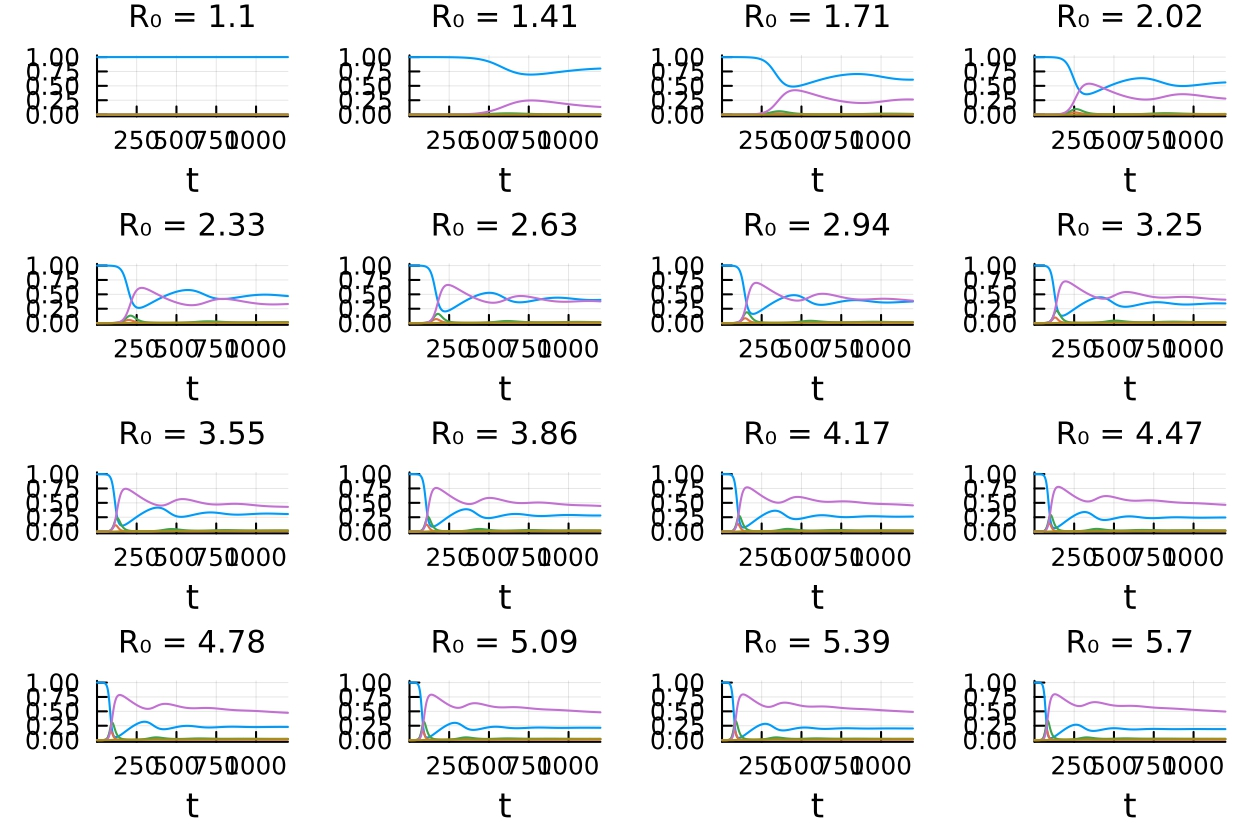
\includegraphics[width=\textwidth]{img/COMPARISON DIFFERENT R0 VALUE_2023-06-29 (1).jpg}
    \captionof{figure}{Comportamento modello SEIR al variare del parametro $R_0$}
    \label{fig:strange_behaviour_R0_ode}
\end{minipage}

Anche se è stata formulata una formula approssimativa per 
descrivere la relazione tra i risultati del modello ABM e SEIR, 
questo comportamento rimane inspiegabile. 

\begin{minipage}{\linewidth}
    \centering
    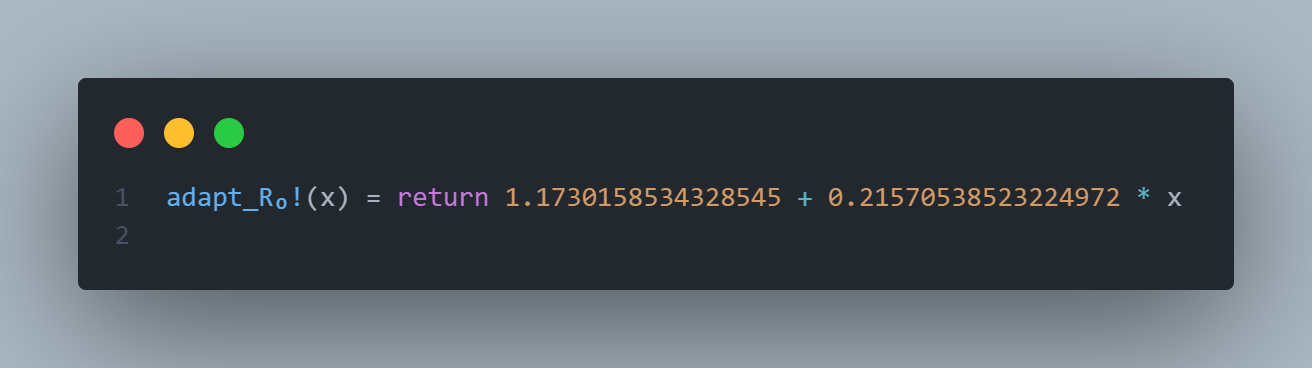
\includegraphics[width=\textwidth]{img/rapporto_strano.png}
    \captionof{figure}{Formula che si occupa di descrivere il rapporto tra il comportamento del modello scartato e del modello SEIR. In particolare questa formula descrive il rapporto tra gli $R_0$}
    \label{fig:strange_behaviour_R0}
\end{minipage}

L'uso di un approccio basato su un grafo e la modellazione del 
singolo agente ha portato a risultati incoerenti e ha reso necessario 
abbandonare questa metodologia a favore di alternative più promettenti.
\newpage

\subsection{Controllore Ipopt}

È stato esplorato un terzo approccio basato su Ipopt 
(Interior Point OPTimizer), un pacchetto software per l'ottimizzazione 
non lineare su larga scala. Ipopt è progettato per trovare soluzioni 
locali a problemi di ottimizzazione matematica, con funzioni obiettivo e 
vincoli non lineari. \cite{Wächter2006}

\begin{minipage}{\linewidth}
    \centering
    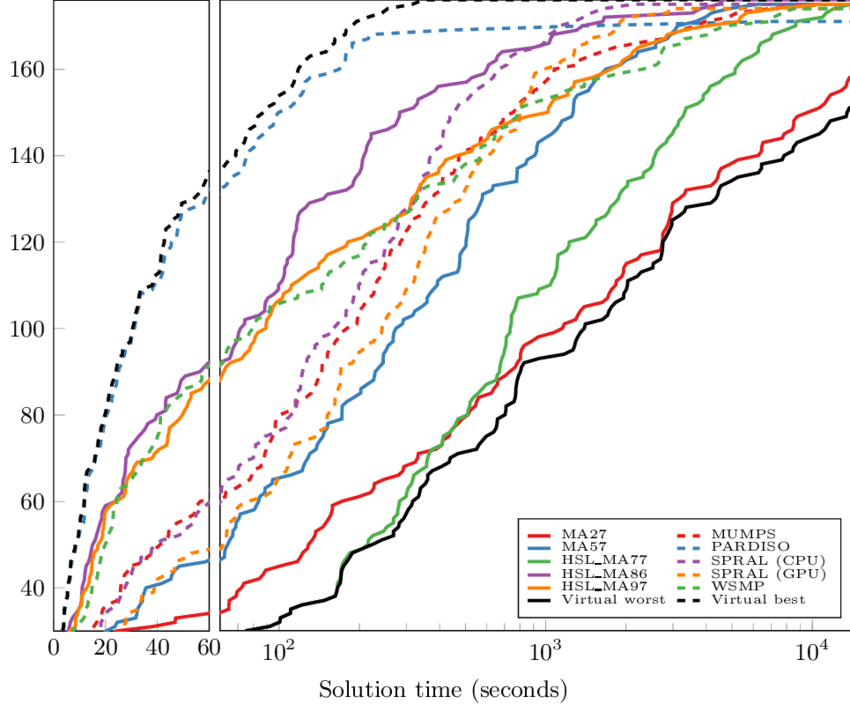
\includegraphics[width=\textwidth]{img/Comparison-of-Ipopt-performance-over-various-linear-solvers-using-the-two-dimensional.png}
    \captionof{figure}{Comparison of Ipopt performance over various linear solvers using the two-dimensional partial differential equation test problem set. \cite{unknown}}
    \label{fig:Ipopt_solver}
\end{minipage}

L'approccio ha previsto l'applicazione di un sistema di 
monitoraggio e intervento all'interno del modello di simulazione, 
con l'obiettivo di ridurre il numero di individui infetti. 
Le regole per il comportamento del modello sono state definite, 
inclusa una rappresentazione degli stati SEIR e un nuovo stato per 
il controllo delle risorse.

\begin{minipage}{\linewidth}
	\centering
	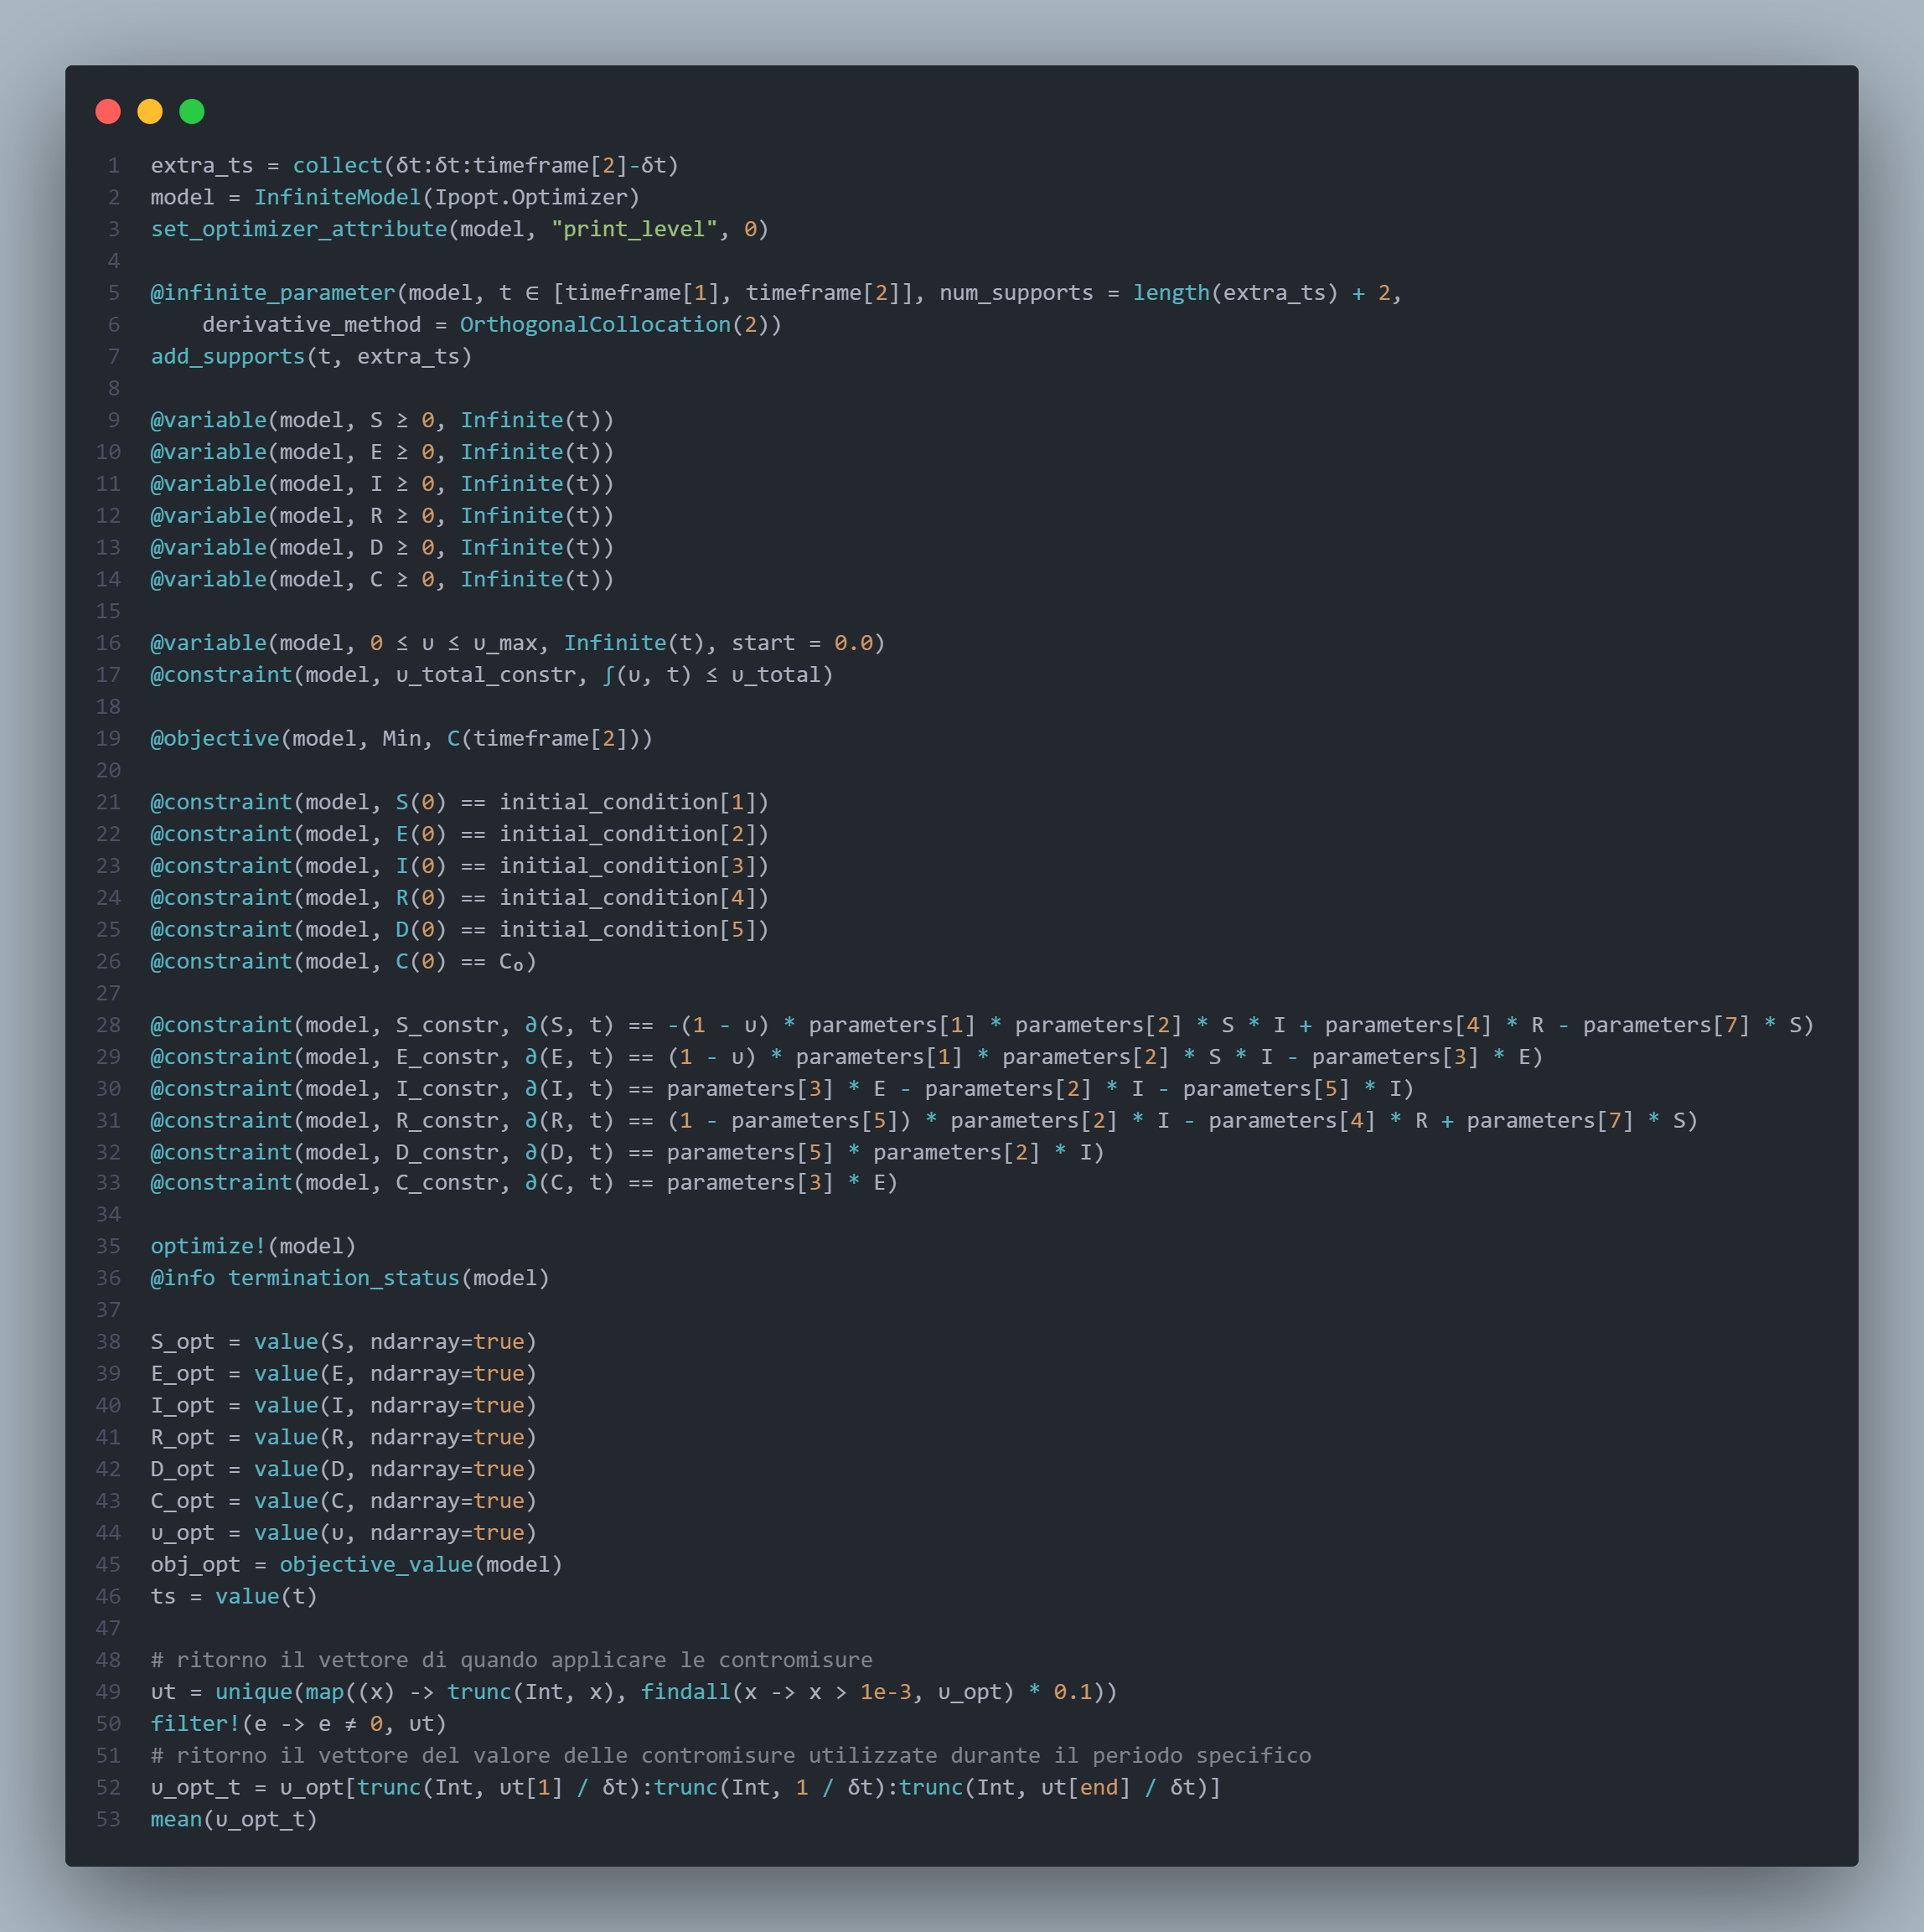
\includegraphics[width=\textwidth]{img/controller_ipopt.png}
	\captionof{figure}{Definizione del controllore tramite Ipopt}
	\label{fig:controller_ipopt}
\end{minipage}

\begin{minipage}{\linewidth}
	\centering
	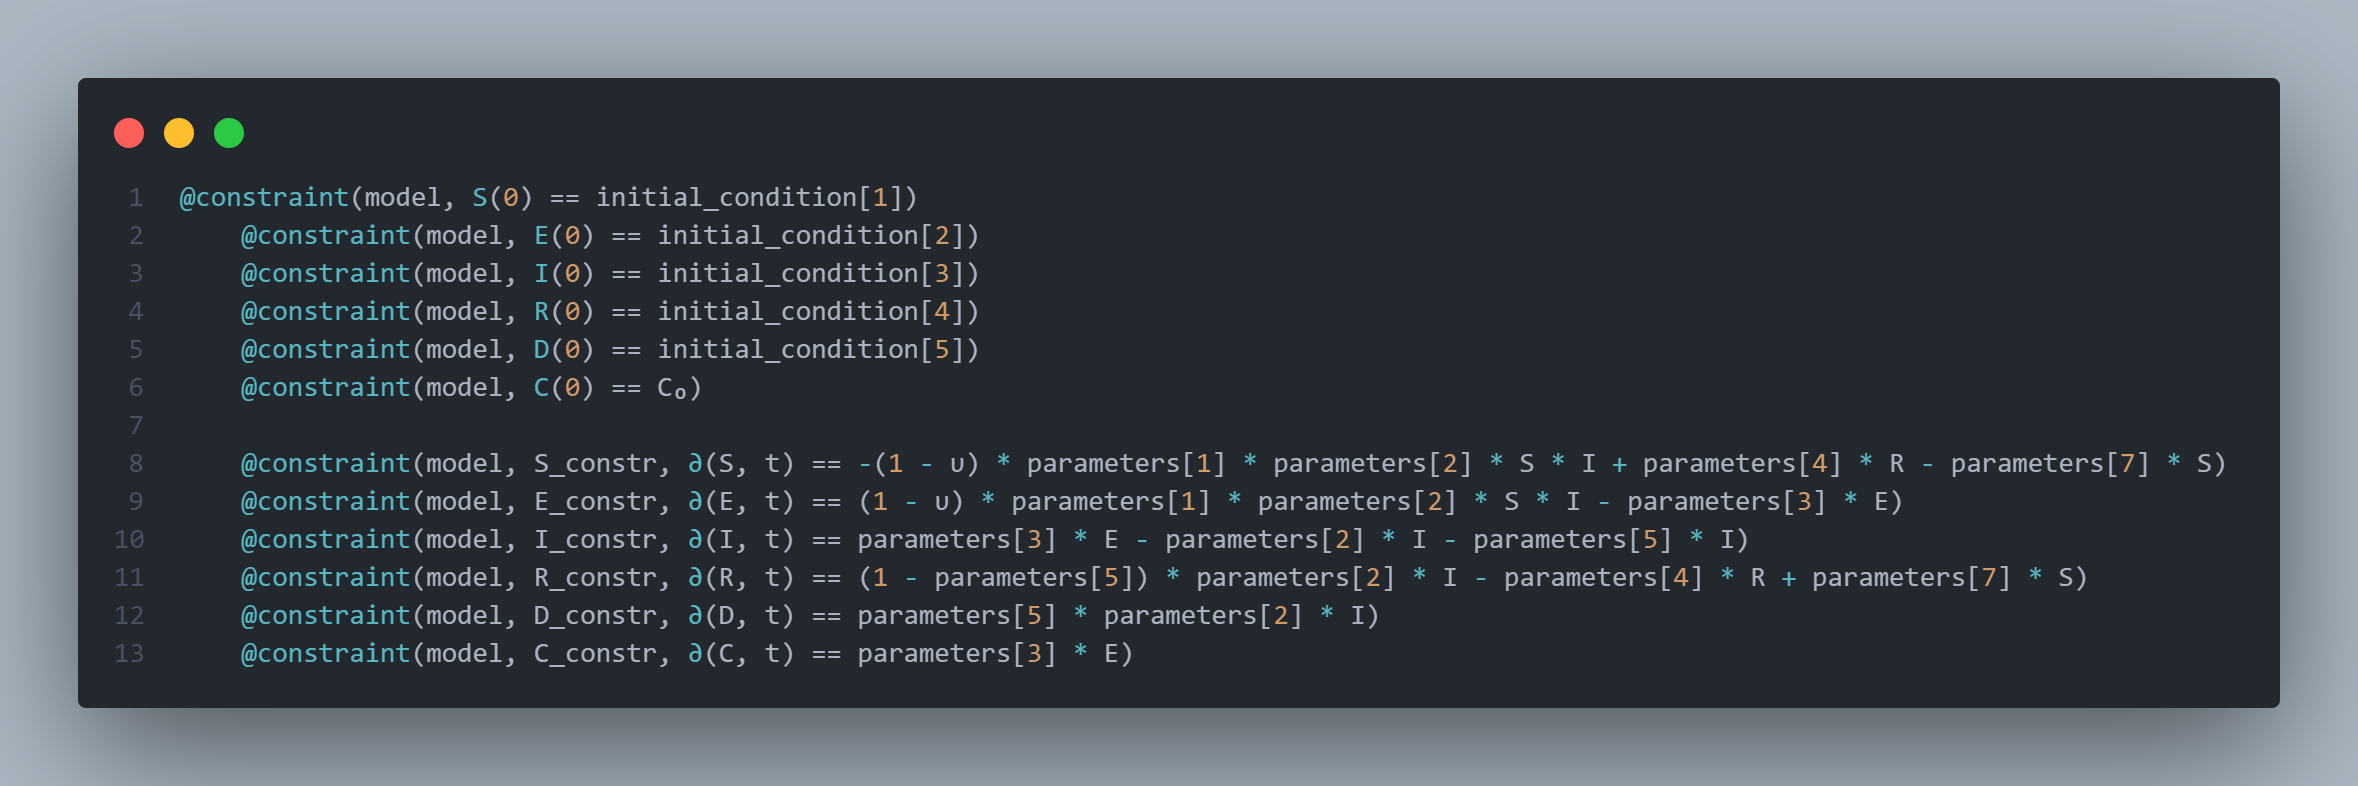
\includegraphics[width=\textwidth]{img/controller_rules.png}
	\captionof{figure}{Definizione regole del modello del controller}
	\label{fig:controller_rules}
\end{minipage}

\begin{minipage}{\linewidth}
	\centering
	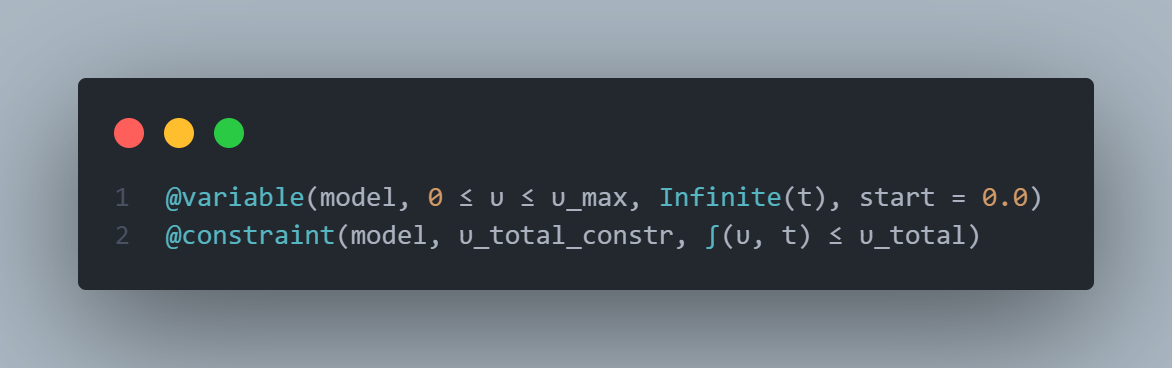
\includegraphics[width=\textwidth]{img/controller_rules_1.png}
	\captionof{figure}{Definizione regole del modello del controller per le contromisure}
	\label{fig:controller_rules_1}
\end{minipage}

Sono state stabilite anche regole per il consumo di risorse, 
rappresentando le contromisure con il loro costo associato. 
L'ottimizzazione del modello è stata eseguita e sono stati restituiti 
i valori medi delle contromisure applicate.

I risultati ottenuti con Ipopt sono stati confrontati con quelli 
dell'implementazione personalizzata, rivelando somiglianze 
significative. Tuttavia, la possibilità di convertire facilmente 
il codice da CPU a GPU è stata determinante nella decisione di 
utilizzare l'implementazione personalizzata, in previsione di futuri 
miglioramenti delle prestazioni del codice.

\begin{figure}[!hb]
	\centering
	\begin{subfigure}[b]{\textwidth}
		\centering
		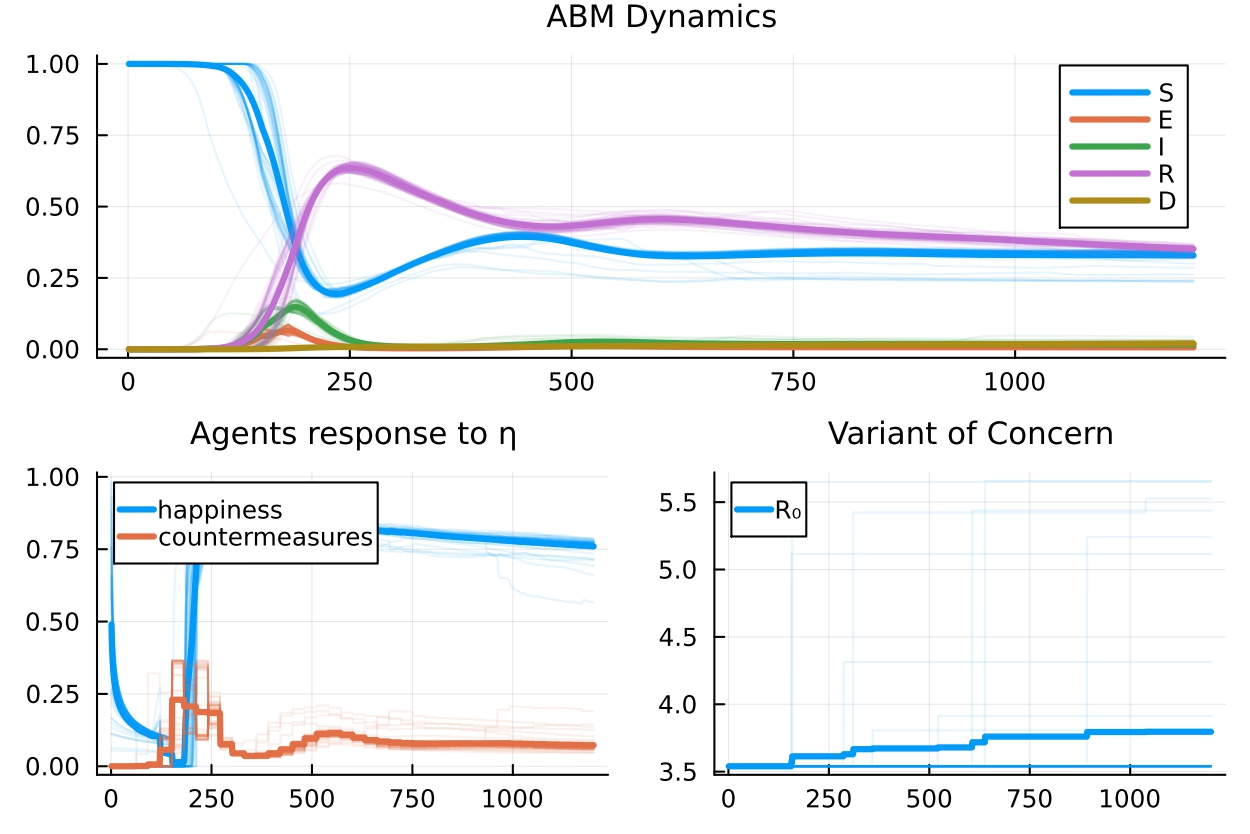
\includegraphics[width=\textwidth]{img/SocialNetworkABM_IPOPT_CONTROL.jpg}
		\caption{Risultato applicazione controllore tramite la suite Ipopt}
		\label{fig:ipopt_res1}
	\end{subfigure}
	\hfill
	\begin{subfigure}[b]{\textwidth}
		\centering
		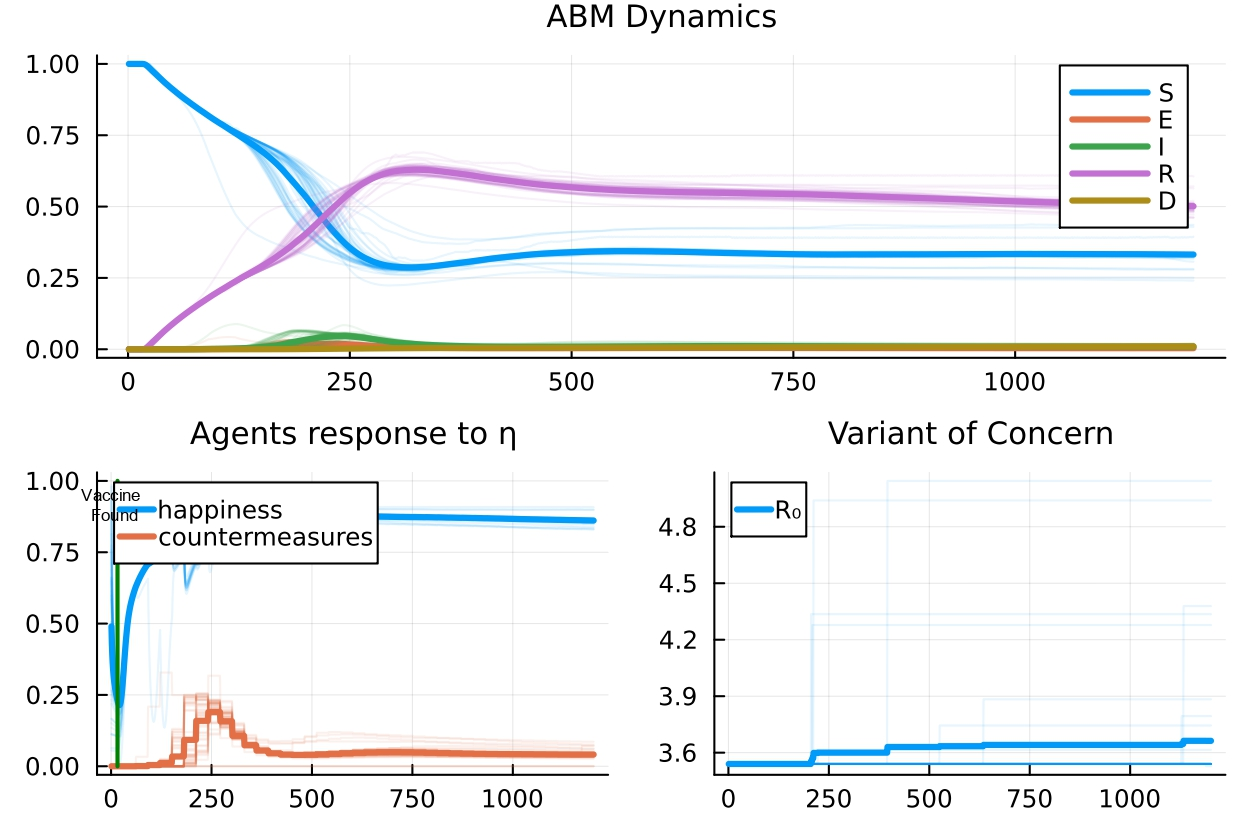
\includegraphics[width=\textwidth]{img/SocialNetworkABM_IPOPT_ALL.jpg}
		\caption{Risultato applicazione controllore tramite la suite Ipopt}
		\label{fig:ipopt_res2}
	\end{subfigure}
\end{figure}

L'approccio ibrido del controllore è stato preferito per la sua 
semplicità e la possibilità di mascherare la funzione obiettivo 
tramite una rete neurale, semplificando notevolmente la definizione 
delle regole rispetto all'implementazione esplicita di Ipopt.